% Beschreibung für den Batch Citation Matcher
% ToDos:
% Workflow beschreiben: Litereraturverzeichnis durchgehen, von den interessanten Artikeln Journalname, Jahr und Autor (angeben)
% Cave: bei mehr als 3 Treffern werden die PMID nicht mehr angegeben, man steht gewissermassen mit "leeren Händen" da.
% Cave: Der BCM reagiert sehr pingelig auf die Angabe unter Journal (ist obligat!). Gelegentlich unterläuft einem ja ein Tippfehler, aber oft sind auch die Abkürzungen in den Literaturverzeichnissen nicht korrekt.


\documentclass[div=15,parskip=half]{scrartcl}
\usepackage[utf8]{inputenc}
\usepackage{lmodern}	% Schrift "Latin Modern"
\usepackage[ngerman]{babel}

\usepackage{keystroke}
\usepackage{url}

\usepackage{graphicx}

\usepackage{hyperref}
\hypersetup{colorlinks=true, linkcolor=blue, urlcolor=blue}
%\pagestyle{empty}	%Auskommentieren, wenn Seitenzahlen gewünscht

\begin{document}

\section*{Schnelles Auswerten von Literaturverzeichnissen: Anleitung für den <<NBCI Batch Citation Matcher>>}
Marco Strehler (\href{mailto:marcostrehler@yahoo.de}{marcostrehler@yahoo.de}). Version vom 25.08.2013.
Die aktuelle Version dieser Anleitung findet sich unter \url{http://de.scribd.com}, Dokument-Nr. 152201179.

\subsection*{Intro}
Ein interessantes Tool auf der NBCI-Website ist der \textsl{Batch Citation Matcher} (Direkter Link: \url{http://www.ncbi.nlm.nih.gov/entrez/getids.cgi}). Damit kann in der Literaturdatenbank mit einen Rutsch nach zahlreichen Einträgen gesucht werden. Das Prinzip: Minimalinformationen werden zeilenweise in ein File geschrieben, dieses hochgeladen und man erhält die \textsl{PubMed Identifiers} (PMID), mit dem die entsprechenden PubMed-Eintrag eindeutig identifiziert sind.

\subsection*{Schritt-für-Schritt}

\begin{enumerate}
	\item Mit einem beliebigen Text-Editor eine neue Datei erstellen.
	\item Zu jedem gesuchten Artikel eine Zeile mit folgenden Format eintippen:
	\begin{verbatim}journal|jahr|volume|erste_seite|autor|schluessel| \end{verbatim}
	Das Feld \textsl{journal} ist obligat, die anderen können ausgelassen werden, allerdings müssen bei weggelassenen Feldern die entsprechenden Feldtrenner ($\vert$) verbleiben\footnote{Das mit dem $\vert$ ist auch wieder eine Sache für sich. Es gibt nämlich zwei verschiedene vertikale Striche. Einer wird (auf der Schweizerdeutschen Tastatur) mit \AltGr-\keystroke{7} und der andere mit \AltGr-\keystroke{1} erzeugt. Der erste ist der richtige.}. Ein weiterer vertikaler Strich wird zusätzlich als Zeilenabschluss benötigt. Als Beispiel eines verkürzten Eintrages mit nur dem Journal-Titel, dem Jahrgang (Volume) und dem Erstautor:
	\begin{verbatim}j consult clin psychol||51||baum|| \end{verbatim}
	Mit dem \textsl{schlüssel} kann ein beliebiger Wert übergeben werden, der bei der Suche ignoriert wird.
	\item Textfile abspeichern
	\item Auf der Seite des \textsl{Batch Citation Matcher} (URL siehe oben) die Datenbank (für unsere Zwecke <<PubMed>>) einstellen, eigene E-Mail-Adresse angeben und das erzeugte Textfile auf der Festplatte auswählen (Knopf <<Durchsuchen>>).
	\item <<Go>> anklicken
	\item Man erhält (nach einiger Zeit, ging bei mir bis zu einer Stunde) eine E-Mail mit dem Output. Der jeweilige PMID ist an der Zeile angehängt. Wenn das Suchkriterium nicht eindeutig war (z.B. wenn eine Autor im selben Jahr mehrere Artikel in der gleichen Zeitschrift veröffentlicht hat), kommen mehrere passende PMID zurück (siehe untenstehende Beispiele).  Der BCM funktioniert nur bei 1:1-Suche. Wenn die Suchkriterien mehrdeutig sind, werden nur drei Treffer geliefert. Bei mehr als drei Fundstellen wird keine mehr angegeben. Auch ist der BCM extrem pingelig bez. Zeitschriften-Abkürzungen.
\end{enumerate}

\subsection*{Beispiel eines Input-Files und für die Rückgabe des BCM}

Inhalt des Input-Text-Files:
\begin{verbatim}
j consult clin psychol||51||baum||
gerontologist||18||bell||
int j aging hum dev||16||bolin||
int j aging hum dev||26||bolin||
gerontologist||21|8|borup||
gerontologist||2||bourestom||
arch gen psychiatry||48||breslau||
\end{verbatim}

Output (erhalten per E-Mail), jeweils mit dem 7-stelligen, angehängten PMID am Ende der Zeilen.

\begin{verbatim}
j consult clin psychol||51||baum||6619364
gerontologist||18||bell||750293
int j aging hum dev||16||bolin||7184870
int j aging hum dev||26||bolin||3338865
gerontologist||21|8|||NOT_FOUND
gerontologist||2||||NOT_FOUND
arch gen psychiatry||48||breslau||AMBIGUOUS 1845224,1996917
\end{verbatim}


\subsection*{Bequemer das Input-File erzeugen mit Hilfe von OpenOffice Calc}

Eine solche Input-Liste anzulegen ist <<von Hand>> mit einem beliebigen Text-Editor möglich. Es geht aber auch konfortabler; und zwar bieteet sich bei solchen strukturierten Eingaben eine Tabellenkalkulation an. Im folgenden am Beispiel von OpenOffice Calc dargestellt.

Zunächst wird in Calc eine neue Tabelle angelegt. In die Spalten A -- E kommen (streng in dieser Reihenfolge) Journal, Jahr, Volume, erste Seite und Erstautor. Wie oben beschrieb ist nur das Journal obligatorisch, die anderen Felder dürfen leer gelassen werden (solange die Publikation damit eindeutig identifiziert werden kann). In die Spalte F kommt der senkrechte Strich ($\vert$). Zur Erinnerung: auf der Schweizerdeutschen Tastatur dargestellt mit \AltGr-\keystroke{7}. Siehe dazu Abbildung \ref{fig:Tabelle}, Seite \pageref{fig:Tabelle}.

\begin{figure}
\label{fig:Tabelle}
\center
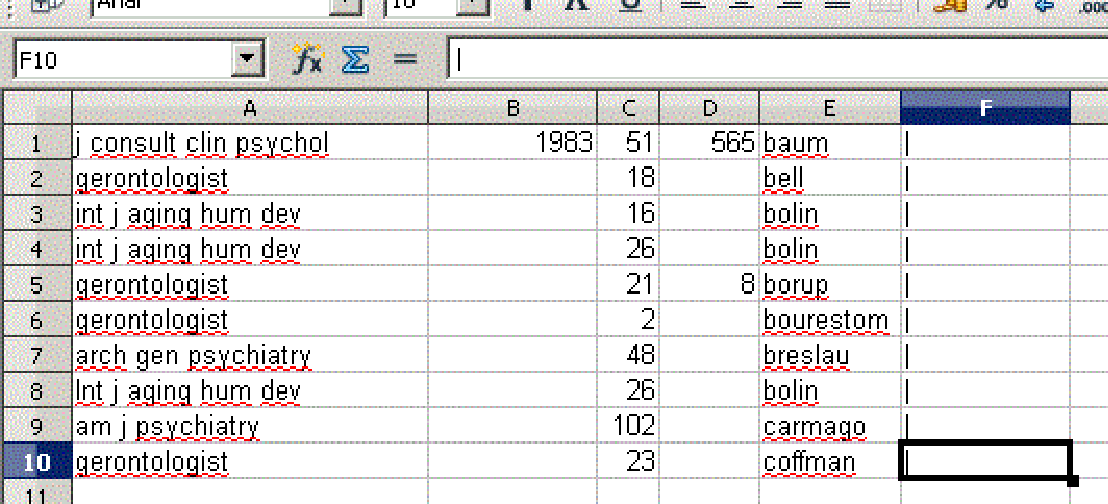
\includegraphics[scale=.7]{fig-oo-calc.pdf} 
\caption{Beispiel, wie die Tabelle in OpenOffice Calc ausgefüllt werden kann. Das Zeichen $\vert$ in der Spalte F ist wichtig und dient dazu, dass beim Abspeichern der Datei im Texformat -- wie vom BCM verlangt -- auch am Zeilenende ein vertikaler Strich steht.}
\end{figure}

Fertig ausgefüllt wird die Tabelle mit <<Speichern unter \dots >> auf der Festplatte abgelegt. Und zwar unter dem Format <<Text CSV (.csv)>>. Im Speichern-Dialog die Optionen <<Automatische Dateinamenerweiterung>> \textbf{deaktivieren} und <<Filtereinstellung bearbeiten>> \textbf{aktivieren}. Als Dateinamen wählt man mit Vorteil ein aussagekräftiger Name. Wichtig ist auch die Extension <<txt>>.

Es erscheint ein Dialog, in dem die Trenner eingestellt werden. Dabei werden die Feld- und Texttrenner gemäss der Abbildung \ref{fig:Filtereinstellung}, Seite \pageref{fig:Filtereinstellung}) eingestellt.

\begin{figure}
\label{fig:Filtereinstellung}
\center
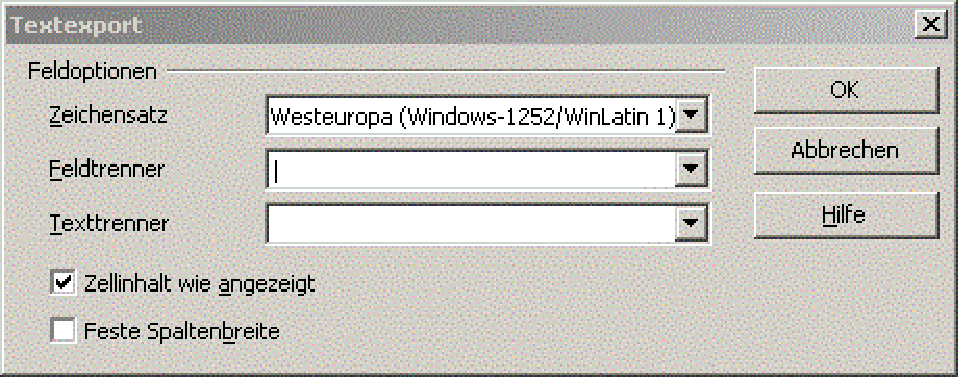
\includegraphics[scale=.7]{fig-filtereinstellung.pdf} 
\caption{Die Filtereinstellung. Feld- und Textrenner können per Menü eingestellt werden, die Voreinstellung muss für unsere Zwecke aber überschrieben werden. Im Feldtrenner kommt der bekannte vertikale Strich und der Texttrenner bleibt leer.}

\end{figure}

\subsection*{PMID und weiter?}

Die PMID kann verwendet werden, um den Eintrag in PubMed direkt zu finden. Dazu kopiert man die Nummer einfach ins Suchfeld. Es kann auch nach mehreren PMID gesucht werden, indem sie mit einem Leerzeichen getrennt eingegeben werden. Wenn also -- ausgehend von obigem Beispiel -- nach folgendem gesucht wird (siehe letzte Zeile im Output):
\begin{verbatim}1845224 1996917 \end{verbatim}
\dots erhält man die zwei entsprechenden PubMed-Einträge (Der Autor \textsl{Breslau} hat in jendem Jahr zwei Artikel im \textsl{Arch Gen Psychiatry} veröffentlicht. 

So kann aber auch direkt aus der entsprechenden Literaturdatenbank (z.B. JabRef) heraus gesucht werden. Mehrfachtreffer und das entsprechende Herausklauben des gesuchten Eintrages entfallen.

\end{document}